\chapter{}
\label{lecture14}
\section[Телеграфные уравнения.]{Дифференциальное уравнение свободных электрических колебаний в проводах.}
\label{lecture14section1}
Пусть по проводнику идёт ток с силой $i(x,t)$ под напряжением $v(x,t)$. При прохождении тока возникает магнитное поле, приводящее к изменениям и напряжения, и силы тока. Возникает колебательный процесс, описываемый некими дифференциальными уравнениями. К выводу этих уравнений мы и переходим. 

Зададим характеристики проводника на единицу длины: $C$ --- ёмкость, $R$ --- сопротивление, $G$ --- утечка, $L$ --- коэффициент самоиндукции (определяет возбуждение электродвижущей силы --- ЭДС --- при изменении силы тока). Пусть $x_1$, $x_2$ --- произвольные точки проводника и направление <<движения>> электронов $x_1\to x_2\to$. 
\vspace{0.2cm}


\tikzset{every picture/.style={line width=0.75pt}} %set default line width to 0.75pt        

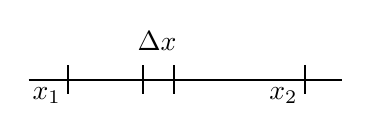
\begin{tikzpicture}[x=0.75pt,y=0.75pt,yscale=-1,xscale=1]
	%uncomment if require: \path (0,124); %set diagram left start at 0, and has height of 124
	
	%Straight Lines [id:da30628681944448344] 
	\draw    (100,54.99) -- (250.89,54.99) ;
	%Straight Lines [id:da65742611183947] 
	\draw    (233,47.86) -- (233,61.86) ;
	%Straight Lines [id:da8272780306530121] 
	\draw    (119,47.9) -- (119,61.9) ;
	%Straight Lines [id:da33223586912832204] 
	\draw    (155,47.9) -- (155,61.9) ;
	%Straight Lines [id:da7985336251753263] 
	\draw    (170,47.9) -- (170,61.9) ;
	
	% Text Node
	\draw (117,57.3) node [anchor=north east] [inner sep=0.75pt]    {$x_{1}$};
	% Text Node
	\draw (231,57.3) node [anchor=north east] [inner sep=0.75pt]    {$x_{2}$};
	% Text Node
	\draw (151,30.39) node [anchor=north west][inner sep=0.75pt]    {$\Delta x$};
	
	
\end{tikzpicture}
\vspace{0.2cm}

Найдём падение напряжения на участке $x_1,\ x_2$. Ясно, что оно определяется для элементарного участка суммой слагаемых, одно из которых $R\cdot i\cdot\Delta x$ отвечает закону Ома, а второе $\displaystyle L\cdot\pder{i}{t}\cdot\Delta x$ --- возникшей ЭДС. Поэтому 
\begin{equation}\label{l14:eq:1}
	\hfill v(x_1,t)-v_(x_2,t)=\int\limits_{x_1}^{x_2}R\cdot i(x,t)\,dx+\int\limits_{x_1}^{x_2}L\cdot\pder{i}{t}\,dx.\hfill
\end{equation}
Записывая
\begin{equation*}
	\hfill v(x_1,t)-v(x_2,t)=\int\limits_{x_2}^{x_1}\pder{v}{x}\,dx=-\int\limits_{x_1}^{x_2}\pder{v}{x}\,dx,\hfill
\end{equation*}
перенесём все члены в~\eqref{l14:eq:1} в одну часть равенства. Получим 
\begin{equation}\label{l14:eq:2}
	\hfill \int\limits_{x_1}^{x_2}\left(\pder{v}{x}+L\cdot\pder{i}{t}+R\cdot i\right)\,dx=0.\hfill
\end{equation}
Так как равенство~\eqref{l14:eq:2} справедливо для любого отрезка $[x_1,x_2]$, то подынтегральное выражение равно нулю и мы получаем первое уравнение
\begin{equation}\label{l14:eq:3}
	\hfill \pder{v}{x}+L\cdot\pder{i}{t}+R\cdot i=0.\hfill
\end{equation}

Далее, падение силы тока на участке $[x_1,x_2]$ связано, во-первых, с тем, что часть зарядов остаётся на этом участке, если действующая на них сила --- напряжение --- меняется во времени. Для элементарного участка $\Delta x$ это  $\displaystyle C\cdot\pder{v}{t}\cdot\Delta x$, а для всего отрезка $[x_1,x_2]$ --- это $\displaystyle\smallint\limits_{x_1}^{x_2}C\cdot\pder{v}{t}\,dx$,	во-вторых, с утечкой части зарядов через поверхность проводника в связи с несовершенной изоляцией. Для элементарного участка $\Delta x$ эта утечка пропорциональна напряжению и равна $G\cdot v\cdot\Delta x$, а для всего отрезка $[x_1,x_2]$ --- это $\displaystyle\smallint\limits_{x_1}^{x_2}G\cdot v\,dx$.
Таким образом 
\begin{equation}\label{l14:eq:4}
	\hfill i(x_1,t)-i(x_2,t)=\int\limits_{x_1}^{x_2}C\cdot\pder{v}{t}\,dx+\int\limits_{x_1}^{x_2}G\cdot v\,dx.\hfill
\end{equation} 
Действуя аналогично предыдущему получаем отсюда
\begin{equation}\label{l14:eq:5}
	\hfill \int\limits_{x_1}^{x_2}\left(C\cdot\pder{v}{t}+\pder{i}{x}+G\cdot v\right)\,dx=0\hfill
\end{equation} 
для любого интервала $[x_1,x_2]$. Следовательно,
\begin{equation}\label{l14:eq:6}
	\hfill C\cdot\pder{v}{t}+\pder{i}{x}+G\cdot v=0.\hfill
\end{equation}  
Уравнения~\eqref{l14:eq:3},~\eqref{l14:eq:6} образуют систему телеграфных уравнений. Считая коэффициенты $C$, $G$, $R$, $L$ --- постоянными, сведём систему~\eqref{l14:eq:3},~\eqref{l14:eq:6} к одному уравнению для этого сначала продифференцируем уравнение~\eqref{l14:eq:3} по $x$, а уравнение~\eqref{l14:eq:6} по $t$. Получим 
\begin{equation}\label{l14:eq:7}
	\hfill \pdder{v}{x}+L\cdot\pder{^2i}{x\partial t}+R\cdot \pder{i}{x}=0,\hfill
\end{equation}
\begin{equation}\label{l14:eq:8}
	\hfill C\cdot\pdder{v}{t}+\pder{^2i}{t\partial x}+G\cdot \pder{v}{t}=0.\hfill
\end{equation} 
Теперь из уравнения~\eqref{l14:eq:7} вычтем уравнение~\eqref{l14:eq:8}, предварительно умножив~\eqref{l14:eq:8} на $L$, чтобы после вычитания полученное уравнение не содержало $\displaystyle\pder{^2i}{t\partial x}$. Получим
\begin{equation}\label{l14:eq:9}
	\hfill \pdder{v}{x}-L\cdot C\cdot\pdder{v}{t}-L\cdot G\cdot \pder{v}{t}+R\cdot \pder{i}{x}=0.\hfill
\end{equation} 
Далее подставим сюда $\displaystyle\pder{i}{x}$ из уравнения~\eqref{l14:eq:6}. В результате придём к уравнению
\begin{equation*}
	\hfill \pdder{v}{x}-L\cdot C\cdot\pdder{v}{t}-L\cdot G\cdot \pder{v}{t}+R\cdot \left(-G\cdot v-C\cdot\pder{v}{t}\right)=0,\hfill
\end{equation*}  
которое запишем в виде
\begin{equation}\label{l14:eq:9a}
	\hfill \pdder{v}{x}=L\cdot C\cdot\pdder{v}{t}+(L\cdot G+R\cdot C)\cdot\pder{v}{t}+R\cdot G\cdot v.\tag{\theequation a}\hfill
\end{equation} 
Если бы мы исключили из системы~\eqref{l14:eq:3},~\eqref{l14:eq:6} не силу тока, а напряжение, то пришли бы к аналогичному~\eqref{l14:eq:9a} уравнению
\begin{equation}\label{l14:eq:10}
	\hfill \pdder{i}{x}=L\cdot C\cdot\pdder{i}{t}+(L\cdot G +R\cdot C)\cdot\pder{i}{t}+R\cdot G\cdot i.\hfill
\end{equation} 
Положим $a_0\eqdef L\cdot C$, $2\cdot b_0\eqdef L\cdot G +R\cdot C$, $c_0\eqdef R\cdot G$ и вместо того, чтобы рассматривать по отдельности каждое из уравнений~\eqref{l14:eq:9a},~\eqref{l14:eq:10} рассмотрим уравнение 
\begin{equation}\label{l14:eq:11}
	\hfill \pdder{w}{x}=a_0\cdot\pdder{w}{t}+2\cdot b_0\cdot\pder{w}{t}+c_0\cdot w,\hfill
\end{equation} 
где $w$ можно понимать как $v(x,t)$, так и $i(x,t)$. В уравнении~\eqref{l14:eq:11} можно избавиться от первой производной по $t$, полагая 
\begin{equation}\label{l14:eq:12}
	\hfill w=e^{-\frac{b_0}{a_0}\cdot t}\cdot u, \hfill
\end{equation}
где $u$ --- новая неизвестная функция. Тогда для функции $u$ мы получим уравнение
\begin{equation}\label{l14:eq:13}
	\hfill \pdder{u}{t}=a^2\cdot\pdder{u}{x}+b^2\cdot u,\hfill
\end{equation} 
где $a=1\!\Bigm/\!\!\sqrt{a_0}$, $b=\sqrt{b_0^2-a_0\cdot c_0}\!\Bigm/\!\!a_0.$

Уравнение~\eqref{l14:eq:13} может быть решено методом разделения переменных без каких-либо затруднений.

Если $b=0$, то уравнение для $u$ совпадает с уравнением свободных колебаний однородной струны. В этом случае говорят, что линия (по которой идёт ток) без искажений (свободна от искажений). Посмотрим, когда это бывает. $b=0$ означает, что $(L\cdot G+R\cdot C)^2=4\cdot C\cdot L\cdot R\cdot G$, откуда 
\begin{equation*}
	\hfill(L\cdot G-R\cdot C)^2=0,\hfill
\end{equation*}
то есть $R\cdot C=L\cdot G$ есть условие отсутствия искажений в линии. Приблизиться к ситуации без искажений можно сделав максимально малыми утечку $G$ и сопротивление $R$.
\section{О начальных и граничных условиях.}
\label{lecture14section2}
Обычно для телеграфных уравнений задаются начальные распределения $i(x,0)$, $v(x,0)$. Однако после сведения системы к уравнению второго порядка нам необходимо знать $\displaystyle\pder{i}{t}(x,0)$ или $\displaystyle\pder{v}{t}(x,0)$ в зависимости от того, что мы берём за $w$ --- силу тока или напряжение. Выручают сами телеграфные уравнения. Из~\eqref{l14:eq:3},~\eqref{l14:eq:6} имеем 
\begin{equation}\label{l14:eq:13a}
	\hfill\pder{i}{t}=\displaystyle\frac{\displaystyle-\left(R\cdot i+\pder{v}{x}\right)}{L},\quad \pder{v}{t}=\displaystyle\frac{\displaystyle-\left(G\cdot v+\pder{i}{x}\right)}{C}.  \hfill
\end{equation}
Полагая здесь $t=0$ мы видим, что правые части~\eqref{l14:eq:13a}, а значит и левые определяются заданием начальных условий. Похожая ситуация с граничными условиями, однако здесь есть подводные камни, на которых мы подробно остановимся. А пока перечислим наиболее часто встречающиеся типы граничных условий. Мы рассматриваем участок провода $[0,l]$.
\begin{enumerateD}
	\item Конец провода заземлён: $v(l,t)=0,\quad\forall t$.
	\item Конец провода изолирован: $i(l,t)=0,\quad\forall t$.
	\item Начало линии находится под синусоидальным напряжением: $v(0,t)=E\cdot\sin\left(\omega\cdot t\right)$.
	\item В начале линии батарея с постоянной электродвижущей силой: $v(0,t)=E$.
\end{enumerateD}

Для того, чтобы получить на обоих концах проводника условия на силу тока или же на напряжение мы можем воспользоваться уравнением~\eqref{l14:eq:3} или уравнением~\eqref{l14:eq:6}. Однако здесь могут возникнуть проблемы, когда начальные и граничные условия рассогласованы. Приведём пример. Пусть дан проводник с начальным распределением силы тока и напряжения по формулам:
\begin{equation}\label{l14:eq:14}
	 i(x,0)=0,\quad v(x,0)=E>0;
\end{equation} 
при $t>0$ левый конец изолировали, а правый заземлили:
\begin{equation}\label{l14:eq:15}
	\hfill i(0,t)=0,\quad v(l,t)=0,\quad t>0.\hfill
\end{equation}  
Мы видим, что начальное и граничное условия для $v(x,t)$ не согласуются: $v(l,0)=E$, а $\displaystyle\lim\limits_{t\to0}v(l,t)=0$. Посмотрим к чему это приведёт. Попробуем найти силу тока $i(x,t)$. Нам надо недостающее начальное условие $\displaystyle\pder{i}{t}(x,0)$. Так как $i(x,0)=0$ и $\displaystyle\pder{v}{x}(x,0)=0$, ибо $v(x,0)$ --- константа, то в силу~\eqref{l14:eq:13a} $\displaystyle\pder{i}{t}(x,0)=0$. Теперь о граничных условиях. На левом конце $i(0,t)=0$, а на правом в силу~\eqref{l14:eq:6} 
\begin{equation}\label{l14:eq:16}
	\hfill\pder{i}{x}=-G\cdot v-C\cdot\pder{v}{t}=0\quad\text{при}\quad x=l. \hfill
\end{equation} 
Таким образом для силы тока мы получаем условия
\begin{equation}\label{l14:eq:17}
	\hfill i(x,0)=0,\quad\pder{i}{t}(x,0)=0,\quad i(0,t)=0,\quad\pder{i}{x}(l,t)=0. \hfill
\end{equation} 
Взяв в~\eqref{l14:eq:11} $w=i$ мы переходим к уравнению~\eqref{l14:eq:13} для $u$. Но $u=w\cdot\exp\left(\frac{b_0}{a_0}\cdot t\right)=i\cdot\exp\left(\frac{b_0}{a_0}\cdot t\right)$ и поэтому для функции $u$ будут в силу~\eqref{l14:eq:17} выполняться нулевые начальные и граничные условия $u(0,t)=0$, $\displaystyle\pder{u}{x}(l,t)=0$. Пусть рассматриваемая линия не имеет искажений ($b=0$). Тогда уравнение~\eqref{l14:eq:13} совпадает с уравнением колебаний струны, для которого доказана теорема единственности решения. Значит $u\equiv0$ и $i(x,t)\equiv0$. Но это невозможно, ибо начальное напряжение равно $E\neq0$. 

\noindent Причина возникшего противоречия заключается в том, что когда в~\eqref{l14:eq:16} мы получили $\displaystyle\pder{i}{x}(l,t)=0$, то это верно лишь при $t>0$, а при $t=0$, во-первых, $v(l,t)=E$, а во-вторых --- и это главное --- $\displaystyle\pder{v}{t}(l,t)$ вообще не существует потому, что функция $v(l,t)$ разрывна в точке $t=0$: 
\begin{equation*}
	\hfill v(l,0)=E,\quad v(l,t)=0,\quad t>0.\hfill
\end{equation*}
Как решать задачу? Есть два подхода. 
\begin{enumerateD}
	\item Сводить к одному уравнению именно для той функции $i(x,t)$ или $v(x,t)$,  для которой имеется несогласованность начальных и граничных условий. В данном случае --- к одному уравнению для $v(x,t)$. В ходе такого сведения для нахождения $\displaystyle\pder{v}{x}(x,0)$ мы будем находить $\displaystyle\pder{i}{x}(x,0)$ (см.~\eqref{l14:eq:13a}), а здесь нет рассогласования и 
	\begin{equation*}
		\hfill \pder{i}{x}(x,0)=0,\quad\text{а }\pder{v}{t}(x,0)=-\frac{G}{C}\cdot E. \hfill
	\end{equation*}
	Недостающее граничное условие на левом конце получаем из~\eqref{l14:eq:3}: $\displaystyle\pder{v}{x}(0,t)=0$. Таким образом мы без проблем свели систему телеграфных уравнений к уравнению относительно напряжения с набором условий:
	\begin{equation*}
		\hfill v(x,0)=E,\quad v_t(x,0)=-\frac{G}{C}\cdot E,\quad \pder{v}{x}(0,t)=0,\quad v(l,t)=0,\quad t>0.\hfill
	\end{equation*}
	Конечно, рассогласованность начального и граничного условий для $v(x,t)$ при $x=l$ не исчезла и поэтому ожидать хорошей сходимости рядов Фурье не приходится.
	
	\item Сглаживание начального условия на маленьком интервале $\eps$ около конца отрезка, решение сглаженной задачи и затем переход к пределу при $\eps\to0$. Или сглаживание граничного условия при $x=l$ на интервале $[0,\eps]$. Другими словами, при наличии рассогласования вводим функции $v_{\eps}(x,t)$, $i_{\eps}(x,t)$ которые кроме телеграфных уравнений подчинены следующим условиям при $t=0$ и на границе: для $i_{\eps}$ --- прежние, 
	\begin{equation}\label{l14:eq:18}
		\hfill v_{\eps}(l,t)=0,\quad v_{\eps}(x,0)=\begin{cases}
			\displaystyle E,& 0\leqslant x\leqslant l-\eps,\\[7pt]
			\displaystyle -\frac{E}{\eps^2}\cdot\Big[x-(l-\eps)\Big]^2+E,&l-\eps\leqslant x\leqslant l. 
		\end{cases}\hfill
	\end{equation} 
	Это сглаживание начального условия. Далее находим $v_{\eps}$ и $i_{\eps}$ и затем $\displaystyle\lim\limits_{\eps\to0}v_{\eps}$, $\displaystyle\lim\limits_{\eps\to0}i_{\eps}$.
	
	Если сглаживать граничные условия для $v(x,t)$, то введя новые неизвестные функции $\widehat{i}_{\eps}$, $\widehat{v}_{\eps}$ мы для них будем иметь прежние телеграфные уравнения и следующие начальные и граничные условия:
	\begin{equation*}
		\hfill \widehat{v}_{\eps}(x,0)=E,\ 0\leqslant x\leqslant l,\quad \widehat{v}_{\eps}(l,t)=\begin{cases}
			0,& t\geqslant\eps,\\[7pt]
			\displaystyle \frac{E}{\eps^2}\cdot(t-\eps)^2,&0\leqslant t\leqslant\eps,
		\end{cases}\qquad \widehat{i}_{\eps}(x,0)=0,\quad\widehat{i}_{\eps}(0,t)=0. \hfill
	\end{equation*} 
	Далее надо найти $\widehat{v}_{\eps}(x,t)$, $\widehat{i}_{\eps}(x,t)$ и перейти к пределу при $\eps\to0$.
\end{enumerateD}  

Заметим, что на практике после нахождения $v_{\eps}$ и $i_{\eps}$ или $\widehat{v}_{\eps}$ и $\widehat{i}_{\eps}$ можно взять значение $\eps$ достаточно малым и получить приближение к решению задачи.